Cada coeficiente complejo obtenido mediante la STFT puede expresarse mediante su magnitud y su fase.
Se obtienen mediante la aplicación de la \textit{transformada en tiempo corto de Fourier}, descrita en la Sección~\ref{sec:stft}, proporciona coeficientes complejos para una serie de celdas con valores de tiempo-frecuencia de una onda. La magnitud es el módulo del coeficiente complejo de la STFT (\textit{Short Time Fourier Transform}, siglas para Transformada de Tiempo corto de Fourier en inglés).

La expresión matemática que representa el módulo o valor absoluto del coeficiente complejo en el dominio tiempo-frecuencia es la siguiente:
\begin{center}    
\( |X(t,f)| \)
\end{center}

Mientras que la fase determina el desfase temporal relativo de esa componente, dependiente del tiempo \textit{t} y de la frecuencia \textit{f}:

\begin{center}
\( \angle X(t,f) \)
\end{center}

En la Figura \ref{fig:OndasPhase} se puede ver un ejemplo de la diferencia de fase (desfase) entre dos ondas sinusoidales desplazadas horizontalmente.
\begin{figure}[H]
    {\begin{center}
    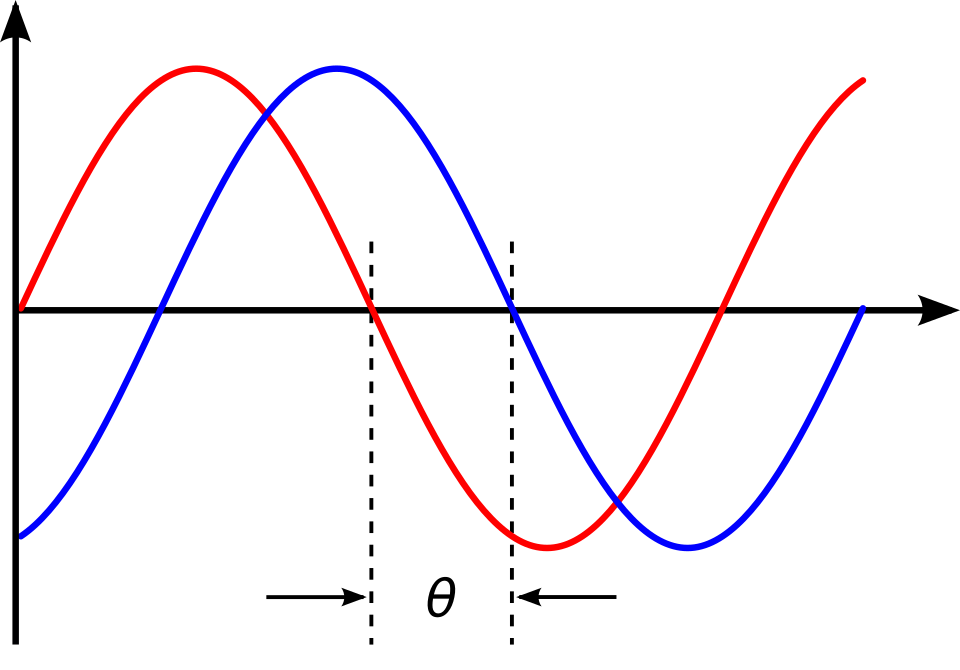
\includegraphics[width=0.7\textwidth]{commons/Phase.png}
    \caption{Diferencia de fase (desfase) entre dos ondas sinusoidales desplazadas horizontalmente.}
    \label{fig:OndasPhase}
    \end{center}}
\end{figure}

Aunque la magnitud es frecuentemente usada como entrada a modelos de separación, la fase es esencial para reconstruir una señal con facilidad, interesante en el contexto del problema que se aborda en este proyecto.